\beginsong{Nun lustig, lustig}[wuw={Werner Helwig}, bo={252}, pfii={75}]

\markboth{\songtitle}{\songtitle}

\beginverse 
\endverse

\centering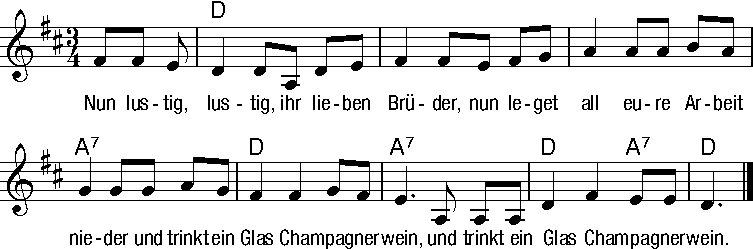
\includegraphics[width=1\textwidth]{Noten/Lied073a.pdf}

\beginverse
Denn unser \[D]Orden, das ist verdorben, die letzten Saufbrüder sind ge \[A7]storben,
\lrep es lebet  \[D]keiner mehr als ich und  \[A7]du. \rrep  \[D]
\endverse

\beginverse
Schifflein, ^Schifflein, nun tu dich wenden und lass dich hin nach Riga ^senden,
\lrep wohl zu der ^russ'schen Seekaufshandels^stadt.\rrep ^
\endverse

\beginverse
Und auch in ^Polen ist nichts zu holen, man kommt von dort nicht unbe^stohlen,
\lrep in Danzig ^fängt die Sauferei schon ^an.\rrep ^
\endverse

\beginverse
Doch wollen ^wir es noch einmal wagen und wollen fahren nach Kopen^hagen,
\lrep wohl zu der ^dänischen Reichsresi^denz. \rrep ^
\endverse

\beginverse
Dann geht es ^heim, wohl an den Main, denn Frankfurt steckt noch voller Äppel^wein,
\lrep der letzte ^Heller muss versoffen ^sein. \rrep ^
\endverse

\beginverse
Denn wer das ^alles hat gesehen, der kann getrost nach Hause ^gehen
\lrep und nehmen ^sich ein junges ^Weib. \rrep ^
\endverse


\endsong

\beginscripture{}
%Nix gefeunden
\endscripture

\begin{intersong}
\ifthenelse{\boolean{pics}}{
\ThisLRCornerWallPaper{1}{Bilder/nunlustig.png}
}{}

\end{intersong}